\documentclass[xcolor=dvipsnames, notes=hide]{beamer}
%\documentclass[xcolor=dvipsnames, notes=only]{beamer}
%\documentclass[xcolor=dvipsnames]{beamer}
%\setbeameroption{show only notes}
%\usepackage{pgfpages}
%\setbeamertemplate{note page}[plain]
%\setbeameroption{show notes on second screen=right}

\usepackage[english]{babel}
\usepackage[utf8]{inputenc}
\usepackage[T1]{fontenc} % Ligaturen, richtige Umlaute im PDF

\newcommand{\backupbegin}{
	\newcounter{finalframe}
	\setcounter{finalframe}{\value{framenumber}}
}
\newcommand{\backupend}{
	\setcounter{framenumber}{\value{finalframe}}
}

\usepackage[absolute,overlay]{textpos} % textblock for figure placement

\usepackage{tabularx, booktabs}
\usepackage{amsmath}
\usepackage{blkarray, bigstrut}
\usepackage{xparse}

\usepackage[normalem]{ulem} % for \sout{}
\usepackage[ruled]{algorithm}
\usepackage{algpseudocode} 
\makeatletter
\def\BState{\State\hskip-\ALG@thistlm}
\algdef{SE}[DOWHILE]{Do}{doWhile}{\algorithmicdo}[1]{\algorithmicwhile\ #1}
\makeatother

\beamertemplatenavigationsymbolsempty
%\selectlanguage{english}
%\usepackage{biblatex}
%\bibliography{Bibliography}

\usepackage{bbm} % For mathbb{1}
\usepackage{csquotes}
\usepackage{colordvi}
\usepackage{xcolor}
%\usepackage{foiltex}

%\usepackage{enumitem}

\usepackage{tikz}
\usetikzlibrary{positioning}
\graphicspath{{/images/}}


\usetheme{CambridgeUS}
% Other valid themes
%   Antibes, Bergen, Berkeley, Berlin, Copenhagen
%   Darmstadt, Dresden, Frankfurt, Goettingen, Hannover
%   Ilmenau, JuanLesPins, Luebeck, Madrid, Malmoe
%   Marburg, Montpellier, PaloAlto, Pittsburgh, Rochester
%   Singapore, Szeged, Warsaw, boxes, default

%\usecolortheme{beetle}
%\usecolortheme{dolphin}
% Other valid color schemes
%    albatross, beaver, beetle, crane, dolphin
%    dove, fly, lily, orchid, rose, seagull
%    seahorse, whale and the one and only wolverine

%%%%%%%%%%%%%%%%%%%%%%%%%%%%%%%%
%%%%% PyCharm Color Scheme %%%%%
%%%%%%%%%%%%%%%%%%%%%%%%%%%%%%%%

%%% COLOR DEFINITIONS
\definecolor{uniBonnBlueDark}{HTML}{004F9F}
\definecolor{uniBonnYellow}{HTML}{F4B400} % lighter shades: FFDE85, FFD35C

\definecolor{pyCharmBgMain}{HTML}{2B2B2B} % RGB: 43, 43, 43

\definecolor{titleCardBg}{HTML}{CFCFEF} % former: F6511D (orange), CFCFEF (light purple) 

\definecolor{pyCharmBgSecond}{HTML}{313335}
\definecolor{pyCharmFgSecond}{HTML}{9F9FAF} % RGB: 159, 159, 175

\definecolor{pyCharmGreen}{HTML}{499C54} % RGB: 73, 156, 84
\definecolor{bfseriescolor}{HTML}{499C54}

%%% Original PyCharmColors:
%\definecolor{pyCharmBgMain}{HTML}{2B2B2B}
%\definecolor{pyCharmFgMain}{HTML}{88B1AC}
%\definecolor{pyCharmBgSecond}{HTML}{313335}
%\definecolor{pyCharmFgSecond}{HTML}{5D5F53}
%\definecolor{pyCharmGreen}{HTML}{499C54}

%%% COLOR SETTINGS
%\setbeamercolor{background canvas}{fg=pyCharmFgSecond, bg=pyCharmBgMain}
%\setbeamercolor{background}{fg=pyCharmFgSecond, bg=pyCharmBgMain}
%
%\setbeamercolor{normal text}{fg=pyCharmFgSecond,bg=pyCharmFgSecond}
%\setbeamercolor{alerted text}{fg=red}
%
\setbeamercolor{palette primary}{fg=pyCharmBgSecond, bg=white}
\setbeamercolor{palette secondary}{fg=pyCharmBgSecond, bg=white}
\setbeamercolor{palette tertiary}{fg=uniBonnBlueDark, bg=white}
%
\setbeamercolor{frametitle}{bg=titleCardBg, fg=uniBonnBlueDark} % Frametitle on every slide
\setbeamercolor{title}{fg=black, bg=titleCardBg}	% Title card slide
%
%\setbeamercolor{local structure}{fg=pyCharmGreen} % light green
%\setbeamercolor{subsection in toc}{bg=pyCharmBgMain, fg=pyCharmGreen}
%\setbeamercolor{section in toc}{bg=pyCharmBgMain, fg=pyCharmGreen}
%
%% For figure captions
%\setbeamercolor{caption}{fg=pyCharmFgSecond}
\setbeamercolor{caption name}{fg=pyCharmGreen}
%
%\setbeamertemplate{itemize item}{fg=pyCharmGreen$\blacksquare$}
%\setbeamertemplate{itemize subitem}{\color{499C54}$\blacksquare$}
%\setbeamertemplate{itemize items}[default]
%\setbeamertemplate{enumerate items}[default]

\setbeamertemplate{section in toc}{%
	{\color{pyCharmGreen} \inserttocsectionnumber.}\color{pyCharmFgSecond}~\inserttocsection}
\setbeamertemplate{subsection in toc}{%
	\hspace{1.2em}{\color{pyCharmGreen}\rule[0.3ex]{3pt}{3pt}} ~\inserttocsubsection\par}

\renewcommand{\textbf}[1]{{\bfseries\color{bfseriescolor}#1}}
%
\setbeamercolor*{palette tertiary}{bg=uniBonnBlueDark}

%%% Numbersets
\newcommand{\eye}{\mathbb{1}} % Identitiy matrix
\newcommand{\one}{\textbf{1}} % One-vector (1 1 ... 1)
\newcommand{\IN}{\mathbb{N}} % Natural numbers
\newcommand{\IR}{\mathbb{R}} % Real numbers
\newcommand{\IZ}{\mathbb{Z}} % Integers
\newcommand{\IQ}{\mathbb{Q}} % Rational numbers
\newcommand{\ID}{\mathbb{D}} % Dyadic numbers
\newcommand{\IC}{\mathbb{C}} % Complex numbers
\newcommand{\IF}{\mathbb{F}} % (Vector) Field
%\newcommand{\vA}{\mathcal{A}}
%\newcommand{\vD}{\mathcal{D}}
%\newcommand{\vB}{\mathcal{B}}
%\newcommand{\vP}{\mathcal{P}}
%\newcommand{\vJ}{\mathcal{J}}
%\newcommand{\vU}{\mathcal{U}}
%%% Basic operators
\newcommand{\IP}{\mathbb{P}} % Probability operator
\newcommand{\IE}{\mathbb{E}} % Expectation operator
\newcommand{\vF}{\mathcal{F}} % Fourier transform
%%% Distributions
\newcommand{\vN}{\mathcal{N}} % Normal distribution
\newcommand{\Bin}{\mathop{\mathrm{Bin}}} % Binomial distribution
\newcommand{\Poi}{\mathop{\mathrm{Poi}}} % Poisson distribution
%%% Others
\newcommand{\Cov}{\mathop{\mathrm{Cov}}} % covariance
\newcommand{\co}{\mathop{\mathrm{co}}} % covariance
\newcommand{\Var}{\mathop{\mathrm{Var}}} % variance
\newcommand{\norm}[1]{\left\lVert#1\right\rVert} % norm
\newcommand{\var}[1]{{\ttfamily#1}} % variable
\newcommand{\tr}{\mathop{\operatorname{tr}}} % trace
\newcommand{\rk}{\mathop{\operatorname{rk}}} % rank
\newcommand{\diag}{\mathop{\operatorname{diag}}} % diagonal
\renewcommand{\vec}[1]{\bm{#1}} % vector
\newcommand{\mat}[1]{\bm{#1}} % matrix
\newcommand{\ten}[1]{\bm{\mathcal{#1}}}
\newcommand{\inv}[1]{#1^{-1}} % inverse
\newcommand{\trn}[1]{#1^\intercal} % transpose
\newcommand{\opt}[2]{#1 \trn{#2}} % outer product
\newcommand{\ipt}[2]{\trn{#1} #2} % inner product
\newcommand{\angles}[2]{\langle #1, #2 \rangle} % scalar product
\newcommand{\Angles}[2]{\bigl \langle #1, #2 \bigr \rangle} % big scalar product
\newcommand{\st}{\operatorname{s.\!t.}} % 'such that'
%%% Stacked symbols
\newcommand{\amin}[1]{\operatorname*{argmin}_{#1}}
\newcommand{\amax}[1]{\operatorname*{argmax}_{#1}}
\newcommand{\sign}{\mathop{\mathrm{sign}}}
\newcommand{\eqex}{\mathop{\stackrel{!}{=}}}
\newcommand{\geex}{\mathop{\stackrel{!}{\ge}}}
\newcommand{\leex}{\mathop{\stackrel{!}{\le}}}
\newcommand{\softmax}{\operatorname*{softmax}}
%%% Table colors
\newcommand\cellr{\cellcolor{red!20}}
\newcommand\cellg{\cellcolor{green!10}}
\newcommand\cellb{\cellcolor{blue!10}}
\newcommand\cello{\cellcolor{orange!10}}
%%% Sets
\newcommand{\set}[1]{\{{#1}\}}
\newcommand{\Set}[1]{\big\{{#1}\big\}}
\newcommand{\BigSet}[1]{\Big\{{#1}\Big\}}
%%% Multisets
\newcommand{\mset}[1]{\{\mskip-5mu\{{#1}\}\mskip-5mu\}}
\newcommand{\Mset}[1]{\big\{\mskip-5mu\big\{{#1}\big\}\mskip-5mu\big\}}
\newcommand{\BigMset}[1]{\Big\{\mskip-5mu\Big\{{#1}\Big\}\mskip-5mu\Big\}}
%%% Footnote
%\deffootnote{1.5em}{1em}{\makebox[1.5em][l]{\thefootnotemark}}

%%% LOGO PLACEMENT
\addtobeamertemplate{frametitle}{}{%
	\begin{tikzpicture}[remember picture,overlay]
	\node[anchor=north east,yshift=-3pt] at (current page.north east) {
		
\includegraphics[height=0.8cm]{images/UNI_Bonn_Logo_Standard_RZ_XL.png}
		
\includegraphics[height=0.8cm]{images/AG_logo_hp_70x70.png}
	};
	\end{tikzpicture}}
%\addtobeamertemplate{frametitle}{}{%
%	\begin{tikzpicture}[remember picture,overlay]
%	\node[anchor=north east,yshift=-9pt] at (current page.north east) {
%		
\includegraphics[height=0.8cm]{images/UNI_Bonn_Logo_Standard_RZ_XL.png}
%		
\includegraphics[height=0.8cm]{images/AG_logo_hp_70x70.png}
%	};
%	\end{tikzpicture}}
% !Tex spellceck = en_US
\usepackage[
	backend=biber,
	%	style=authoryear-icomp,
	sortlocale=en_US,
	natbib=true,
	url=false, 
	doi=true,
	eprint=false
]{biblatex}
\addbibresource{../../../bib_file_THESIS.bib}

\title[Master thesis - Handout]{
	\centering
	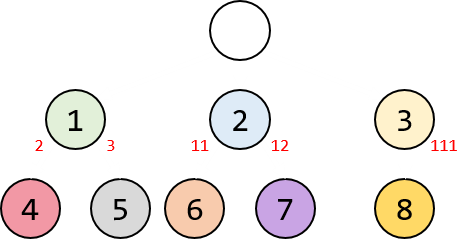
\includegraphics[width=0.3\textwidth]{images/WLLT}\\
	Master Thesis - Handout
}
\subtitle{\enquote{Learning Graph Similarities\\Using The Weisfeiler-Leman Label Hierarchy}}
\author[F. Beaumont]{Fabrice Beaumont}
\institute[]{Department of Information Systems and Artificial Intelligence\\\textbf{Dr. Pascal Welke}}
\date{10. November 2022}

\newcommand{\figureWidth}{7cm}
\newcommand{\figureHorizontal}{2cm}
\newcommand{\figureVertical}{5cm}\begin{document}

\begin{frame}
	\titlepage
\end{frame}

%%%%%%%%%%%%%%%%%%%%%%%%%%%%%%%%%%%%%%%%%%%%%%%%%%%%%%%%%%%%%%%%%%%%%%%%%
\section{Research question}

\begin{frame}
\frametitle{Formal statement of the thesis project}
	In my thesis, I am going to\\
	investigate the effect of learning similarities between Weisfeiler Leman labels and using these in the definition of a \textbf{graph similarity measure},\\
	structured similarly to the Wasserstein Weisfeiler Leman graph kernel proposed in 2019 by Togninalli et al.~\cite{2019_Togninalli_NIPS}.\\
	
	The goal is to discuss, whether learning such similarities can improve the flexibility of the resulting graph similarity measure.
	The machine learning will be restricted in the sense that the ground distance is set as a a tree metric on the Weisfeiler Leman label hierarchy tree. 
	The learning procedure includes iterative updates to the edge weights in this tree. Thereby changing the resulting distance between the Weisfeiler-Leman labels used for the similarity computation.
\end{frame}

%%%%%%%%%%%%%%%%%%%%%%%%%%%%%%%%%%%%%%%%%%%%%%%%%%%%%%%%%%%%%%%%%%%%%%%%%
\section{Definitions}

\begin{frame}[allowframebreaks=0.9]
\frametitle{Definitions on graphs}
	We define a \textbf{graph} as a tuple $G=(V, E)$, where $V$ denotes a finite set of vertices and $E\subseteq 2^V$ a finite set of sets of edges on $V$. 
	We also write $V(G)$ to refer to the vertex set of a graph $G$.
	In this thesis we consider edges to be undirected. 
	That is an edge is a set of two distinct vertices:
	\begin{equation}
		E=\big\{ \{v,w\}| v\neq w \;\land\; v,w\in V \big\}
	\end{equation}
	Such graphs are sometimes called undirected simple graphs.
	Two graphs $G_1$ and $G_2$ are \textbf{isomorphic}, if there exists a bijective function between their vertices, that preserves all edges, and vertex labels.
	If for a graph $G=(V, E)$ and subsets $V^\prime \subseteq V$ and $E^\prime \subseteq E$ the tuple $T^\prime=(V^\prime, E^\prime)$ is also a graph, we call it \textbf{subgraph} of $G$.
	We say a graph is \textbf{labeled}, if its vertices have categorical labels.
	These are denoted by a function $L:V\to\Sigma$ for a finite alphabet $\Sigma$~\cite{2019_Togninalli_NIPS}.
	In the context of this thesis, we will have natural numbers as labels, such for an $s\in \IN$ it is $\Sigma = [-1, s]\subseteq\IN$.
	$G$ is called attributed, if there exists a vertex attribute function $a: V \to\IR$.
	We say a graph is \textbf{weighted}, if there is a weight function $w:E\to\IR$ on the edges of the graph.
	In the context of this thesis, we will have natural numbers as labels, such that there exists an $s\in \IN$ such that $\Sigma = [-1, s]$.  
	When $G$ is clear from the context, denote the number of vertices as $n:=|V|$ and the number of edges as $m:=|E|$.\\
	
	Let $G$ be a graph. 
	We define a \textbf{walk} $\mathcal{W}(v_1, v_{k+1})$ in $G$ from vertex $v_1\in V$ to vertex $v_{k+1}\in V$ as a sequence of edges and vertices $\mathcal{W}(v1, v_{k+1}) = \{ v_1, e_1, v_2,\allowbreak\dots v_k, e_{k}, v_{k+1} \}$ where $e_i=\{v_i, v_{i+1}\}\in E$ for $i=1,\dots,k$. 
	The \textbf{length of this walk} is denoted $|\mathcal{W}(v_1, v_{k+1})|=k$.
	Given a weighted graph $G=(V,E)$ with weight function $w:E\to\IR$, we define the \textbf{distance} $d_G(v,w)$ between two vertices $v$ and $w$ in $G$ as the sum of all weights of all edges in the $\mathcal{P}(v,w)$:
	\[ d_G(v,w) = \sum_{e\in \big( \mathcal{P}(v,w) \cap E\big) } w(e) \]
	A graph $G$ is called connected, if for every two vertices $v$ and $w$ there exists a walk $\mathcal{W}(v, w)$ in $G$.
	For a vertex $v\in V$ in a graph $G=(V, E)$ we define its \textbf{neighborhood} $\mathcal{N}(v)$ as the set of vertices (\textbf{neighbors}) $n$ such that there exists an edge $e=\{v, n\}\in E$ between $v$ and $n$ (which is a path $\mathcal{P}(v,n)$ of length zero)~\cite{2019_Togninalli_NIPS}:
	\[ \mathcal{N}(v) = \{ u\in V | \ \{u,v\}\in E  \} \]
	More generally we define the $k$\textbf{-th-order neighborhood} $\mathcal{N}_k(v)$ of a vertex $v\in V$ in a graph $G=(V, E)$ as the set of vertices ($k$-th-order neighbors) $n$ such that there exists a walk $\mathcal{W}(v,n)$ of length of at most $k$:
	\[ \mathcal{N}_k(v) = \{ u\in V | \ |\mathcal{W}(v, k)| \le k  \} \]
	Notice that $\mathcal{N}(v) = \mathcal{N}_1(v)$ and for $k>1$, $\mathcal{N}(v)\neq \emptyset$ implies $v\in \mathcal{N}_k(v)$.
	The \textbf{degree} $\delta(v)$ of a vertex $v \in V$ is given as the size of its first neighborhood, that is $\delta(v):= |\mathcal{N}(v)|$.\\
	
	We define a \textbf{path} $\mathcal{P}(v_1, v_{k+1})$ as a walk $\mathcal{W}(v_1, v_{k+1})$ such that no vertex or edge in the walk equals another ($e_i\neq e_j$ for all $1\le i<j\le k$ and $v_i\neq v_j$ for all $1\le i<j\le k+1$).
	We define a \textbf{circle} as a walk $\mathcal{W}(v_1, v_{k+1})$ such $v_1 = v_{k+1}$ and no other vertex and no edge equals another.
	We define a \textbf{tree}\label{def:Tree} as a connected graph $T=(V, E)$, which does not contain any circles~\cite{2018_Korte_BOOK}. 
	Notice that this implies that all paths in $T$ are unique. 
	That is there cannot be two different path between two vertices.
	We extend the notion of subgraphs to subtrees.
	A tree $T=(V, E)$ is called \textbf{rooted} if there exists a distinguished vertex $r\in V$ called \textbf{root}.
	In every tree we call vertices with only one adjacent edge (that is a vertex $v$ such that $|\{e\in E:\ v\in e\}|=1$) the \textbf{leaves} of the tree.
	The \textbf{depth} of a vertex $v\in V$ in a rooted tree with root $r$ is defined as length of the path between $v$ and $r$ ($\mathcal{P}(v,r)$).
	We say the root has length zero.
	For two neighboring vertices $v$, $w$ and the edge that connects them $e=\{v, w\}$ we call $v$ the \textbf{parent} of $w$ ($v_p$), if $v$ has smaller depth than $w$.
	$w$ is then called \textbf{child} of $v$ ($v_c$).
	Notice that in this definition $w$ cannot be the root $r$, since no vertex has smaller depth than $r$. 
	Thus the root has no parent and we set $r_p=\emptyset$.
	We extend the definition to the connecting edge $e$ and say $v$ is the parent vertex of $e$ ($e_p=w$) and $w$ is the child vertex of $e$ ($e_c=w$).
	All vertices on the path from $v$ to the root $r$ are called \textbf{ancestors} of $v$.
	We call a tree \textbf{leveled}, if all paths between all leaves and the root have the same length.
\end{frame}

\begin{frame}[allowframebreaks=0.9] \frametitle{Definitions on tree metrics}
	A metric $d:\Omega\times\Omega\to\IR$ is called a \textbf{tree metric} on $\Omega$ if there exists a tree $T=\{V, E\}$ with non-negative edge weights such that all elements of $\Omega$ are contained in its vertices ($\Omega\subseteq V$) and such that for every $v, w\in\Omega$, one has that $d(v,w) = d_G(v,w)$ equals to the distance between the vertices $v$ and $w$ in $T$~\cite{2019_Le_NIPS}.% Def on page 2, section 2
	In this work we will use tree metrics with $\Omega=V$.
	Also note that we will only consider rooted trees and compute distances between vertices that have equal depth.
	This greatly reduces the actually used domain for our tree metric.
\end{frame}

\begin{frame}[allowframebreaks=0.9] \frametitle{Definitions on the used Wasserstein Distance}
	Let $T=(V, E)$ be a rooted, weighted tree with edge weights $w$, a root $r\in V$ and a tree metric $d_T$.
	We define $\Gamma(x)$ as the set of vertices in the rooted subtree of $T$ that contains $x$ as root and all other vertices have higher depth than $x$ in $T$. 
	That is to say all vertices, such that the unique path $\mathcal{P}(r, z)$ from them to the root $r$ contains the vertex $x$:
	\[ \Gamma(x) := \{ z\in V(T)|\ x\in \mathcal{P}(r, z) \} \]
	%Notice that one requires, that the tree metric $d_T$ can be expressed using a unique Borel measure on $T$ as $d_T(x,y) = \lambda\big( \mathcal{P}(x,y) \big)$ for all $x,y\in V$.
	%Using the length measure as $\lambda$
	Using this, we can define the \textbf{closed form, negative definite Tree Wasserstein Distance} on $T$ in the following way~\cite{2019_Le_NIPS}.% Def.: page 3 
	For two Borel probability distributions $\mu, \nu$ on $V$, the Tree Wasserstein Distance can be computed as
	\[ \mathbb{W}_{d_T}(\mu, \nu) := \sum_{e\in E} w(e) \ \Big|\mu \big( \Gamma(e_c) \big) - \nu \big( \Gamma(e_c) \big) \Big| \]
\end{frame}

\begin{frame} \frametitle{Definitions on Weisfeiler-Leman labels I}
	The \textbf{Weisfeiler-Leman} (WL) \textbf{labeling scheme} is vertex labeling scheme at the center of the Weisfeiler-Leman test of graph isomorphism proposed by Boris Weisfeiler and Andrei Leman~\cite{1968_Weisfeiler_CONF}.
	In this thesis we will consider the $1$-dimensional version of the WL labeling scheme. 
	It is also denoted as WL labeling scheme, $1$-WL vertex embedding, WL color refinement, naive vertex refinement.
	In terms of the higher-dimensional $k$-WL labeling scheme it is equivalent to 2-WL labeling scheme and thus the $2$-variable language with counting~\cite{2011_Shervashidze_JMLR, 2019_Xu_CONF, 1992_Cai_IEEE}. 
	
	The scheme iteratively propagates neighborhood information by compressing it in vertex labels~\cite{1968_Weisfeiler_CONF}.
	These vertex labels will be called WL-labels, where the zeroth WL-labels can also denote original vertex labels.
\end{frame}

\begin{frame} \frametitle{Definitions on Weisfeiler-Leman labels II}
	\begin{algorithm}[H] % TODO: Check remakrs on pdf!
		\caption{WL labeling scheme} \label{alg:WLmethod} 
		\begin{tabbing}
			\textbf{Output:} \= \kill
			\textbf{Input:} \>a graph $G=(V, E, L)$ and\\
			\>a perfect hash function.\\		
			\textbf{Output:} \>a vector representation of $G$ of size $|V|$.
		\end{tabbing}	
		\begin{algorithmic}[1]
			\State $\ell^0(v) \leftarrow \operatorname{hash}(L(v))$ for all $v\in V$
			\State $\big(\ell^{1}(v)\big)_{v\in V} = \emptyset$
			\State $k=1$
			\While {$\big(\ell^{k}(v)\big)_{v\in V} \neq \big(\ell^{k-1}(v)\big)_{v\in V}$}
			\State $\ell^{k}(v) \leftarrow \operatorname{hash}\big(\ell^{k-1}(v), \mset{\ell^{k-1}(w)| \ w\in\mathcal{N}_G(v)} \big)$ for all $v\in V$ \label{line:newWlHash}
			\State $k=k+1$
			\EndWhile		
			\State\Return $\big(\ell^{k-1}(v)\big)_{v\in V}$
		\end{algorithmic}
	\end{algorithm}
\end{frame}

\begin{frame} \frametitle{Definitions on Weisfeiler-Leman labels III}
	The procedure was generalized by \cite{2019_Xu_CONF} with $\ell^0(v) = L(v)$ for labeled graphs and $\ell^0(v) = |\mathcal{N}(v)|$ for unlabeled graphs \cite{2009_Shervashidze_NIPS}.
	However using uniform labels $\ell^0(v) = 0$ for unlabeled graphs results in an equivalent labeling, just delayed by one iteration.
	
	To obtain a maximally powerful embedding, the aggregation and hashing step (line \ref{line:newWlHash}) must be injective~\cite{2019_Xu_CONF}.
	This injective aggregation is often realized by sorting the WL-labels of the neighborhood first.
	For the hash function we will consider the set of integers as its range.
	More precisely, the hash function shall map the given inputs to the next free integer, that is not already the image to an input.
	Notice how WL-labels (of deeper iterations) relate iteratively to the $n$-th order neighborhoods of the vertices.
	Thus comparing two WL-labels relates to comparing complete neighborhoods, similarly to subgraphs.
	More accurately, WL-labels are equivalent to so called unfolding trees.
\end{frame}

\begin{frame}
\frametitle{Weisfeiler Leman labeling scheme}
\centering
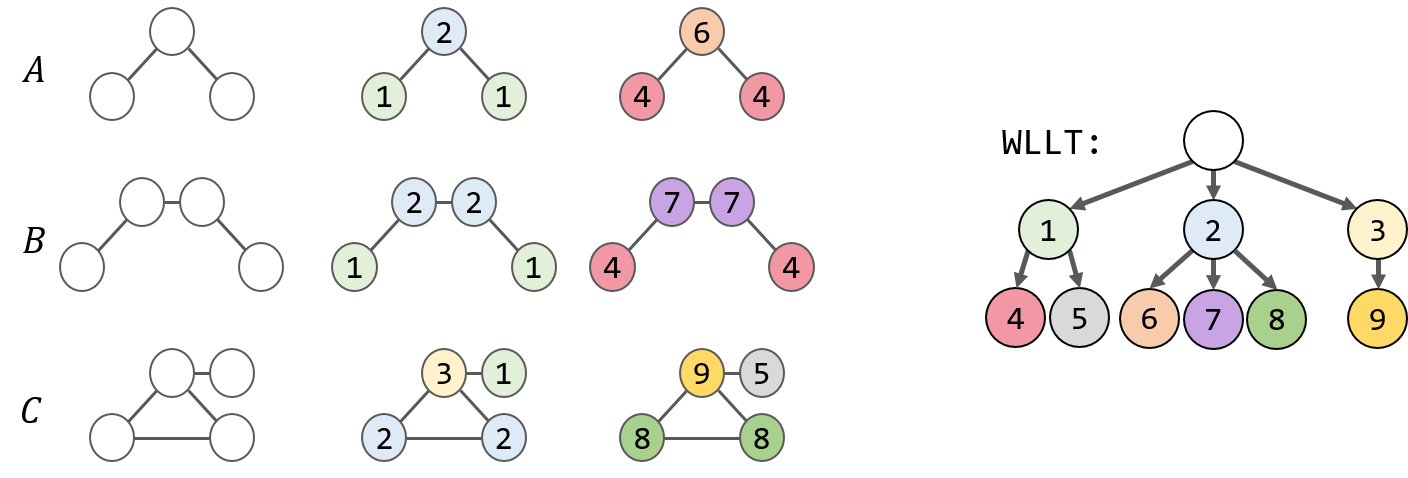
\includegraphics[width=1.0\textwidth]{images/WL_labeling_iterations}
\end{frame}

\begin{frame} \frametitle{Weisfeiler Leman labeling tree I}
	Given $k$ iterations of WL labelings on a database of graphs $\mathcal{G}$, one can construct a WLLT $T$.
	Labeled and un-labeled graphs can be treated in the same way, by considering vertex labels as the zeroth WL-labels.
	With this in mind, use an artificial label to initialize the root of $T$. 
	The $k$-th layer of $T$ consists of all arising WL labels in iteration $k$ of the labeling in any graph .
	That is, there exists an edge $(l,l^\prime)$ in the tree between vertices $l$ and $l^\prime$ if there exists a vertex $v\in V(G)$ in some graph $G\in\mathcal{G}$ and $k\in\IN$ with $l=\ell^k(v)$ and $l^\prime=\ell^{k+1}(v)$.
	The complete construction of the WLLT is sketched in algorithm \ref{alg:WLLTconstruction}.
\end{frame}

\begin{frame} \frametitle{Weisfeiler Leman labeling tree II}	
	The $k$-th WL label of vertex $v$ is given by $\ell_k(u)$.
	Notice that if two vertices have different WL labels in one refinement step, this implies that they have different WL labels in all later refinement steps~\cite{1968_Weisfeiler_CONF, 2016_Kriege_NIPS}:
	\[ \forall u,v \in V \ \forall i\in \IN: \quad \ell_k(u)\neq \ell_k(v) \implies \ell_{k+1}(u)\neq \ell_{k+1}(v) \]
	Hence the sequence of WL labels gives rise to a hierarchy which can be represented in a tree.
\end{frame}

\begin{frame} \frametitle{Weisfeiler Leman labeling tree III}
	\begin{algorithm}[H]
		\caption{WLLT construction} \label{alg:WLLTconstruction} 
		\begin{tabbing}
			\textbf{Output:} \= \kill
			\textbf{Input:} \>a graph dataset $\mathcal{G}$,\\
			\>WL labeling depth $k$.\\
			\textbf{Output:} \>WLLT $T$ of height $k$ (unweighted).
		\end{tabbing}	
		\begin{algorithmic}[1]		
			\State Initialize the WLLT as a single root $T=({r}, \emptyset)$
			\For {$G$ in $\mathcal{G}$}
			\For {$i=0$ to $k$}
			\State Generate the $i$-th WL-feature $F$ of $G$
			\For {$l\in F$}
			\If {$l\notin T$}
			\State $V(T) = V(T) \cup \{ l \}$
			\State $E(T) = E(T) \cup (p, l)$ where $c^{i-1}(v)=p$ and $c^{i}(v)=l$ 
			\EndIf					
			\EndFor
			\EndFor
			\EndFor
			\State \textbf{return} $T$
		\end{algorithmic}
	\end{algorithm}	
\end{frame}

%%%%%%%%%%%%%%%%%%%%%%%%%%%%%%%%%%%%%%%%%%%%%%%%%%%%%%%%%%%%%%%%%%%%%%%%%
\section{Method}

\begin{frame} \frametitle{Method sketch}
\vspace{-0.75cm}
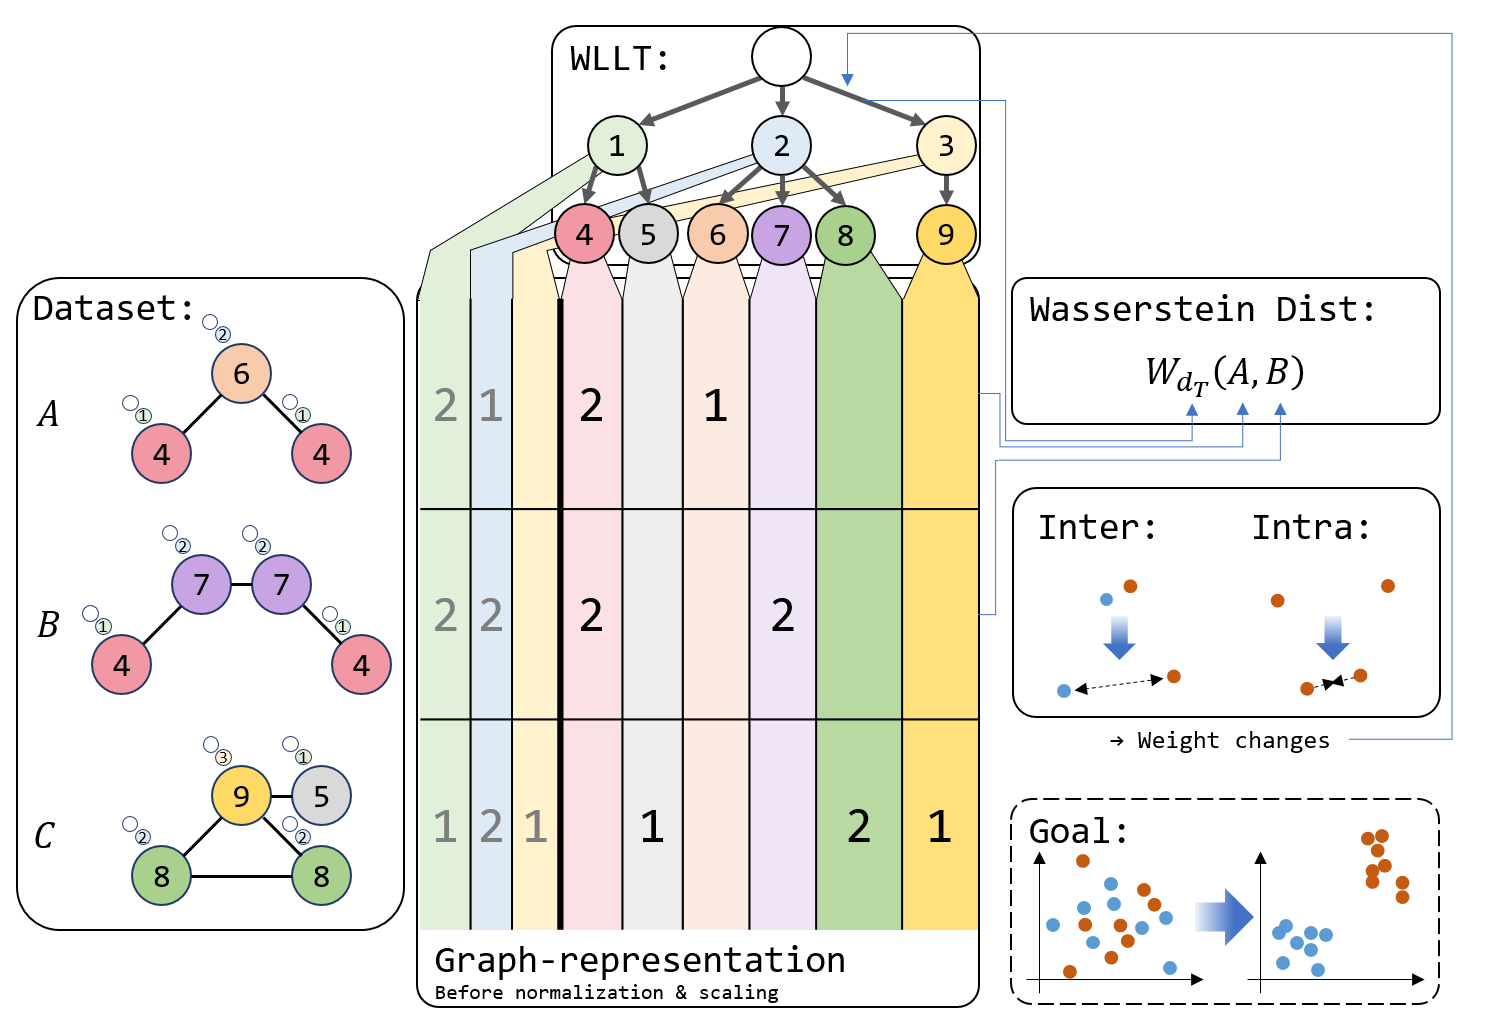
\includegraphics[width=0.95\textwidth]{images/WLLTProgram6}
\end{frame}



%%%%%%%%%%%%%%%%%%%%%%%%%%%%%%%%%%%%%%%%%%%%%%%%%%%%%%%%%%%%%%%%%%%%%%%%%
\section{References}

\begin{frame}[allowframebreaks=0.9]
	\printbibliography
\end{frame}

%%%%%%%%%%%%%%%%%%%%%%%%%%%%%%%%%%%%%%%%%%%%%%%%%%%%%%%%%%%%%%%%%%%%%%%%%
%\appendix
%\section{Appendix}
%
%\begin{frame}[noframenumbering]
%\frametitle{Example of the whole procedure}	
%
%\end{frame}

\end{document}